\chapter{Duality correspondences}
\label{chap:duality_correspondences}

In this chapter we explore various topics which connect to our treatment of 
Lagrangian duality and the KKT conditions in the last two chapters.

\section{Dual norms}
\label{sec:dual_norms}

Given a norm $\|\cdot\|$ on $\R^d$, its \emph{dual norm} is denoted
$\|\cdot\|_*$, and defined by 
\index{dual norm}  
\begin{equation}
\label{eq:dual_norm}
\|y\|_* = \sup_{\|x\| \leq 1} \, y^\T x.
\end{equation}
It is not hard to check that the dual norm $\|\cdot\|_*$ is itself a norm on
$\R^d$, that is, it satisfies the triangle inequality, absolute homogeneity, and
positive definiteness (Exercise \ref{ex:dual_norm_check}). 

A key property to record: the dual of the dual norm is the original norm,
$\|\cdot\|_{**} = \|\cdot\|$. This is traditionally verified using the
Hahn-Banach theorem (Exercise \ref{ex:dual_norm_dual1}), but can also be
derived using the theory of Lagrangian duality (Exercise
\ref{ex:dual_norm_dual2}), or even convex conjugacy (Exercise
\ref{ex:dual_norm_dual3}). In any case (however it is proved), this fact allows 
us to write    
\begin{equation}
\label{eq:norm_dual2}
\|x\| = \sup_{\|y\|_* \leq 1} \, x^\T y.
\end{equation}

Directly from \eqref{eq:dual_norm}, we may infer that $x^\T y \leq \|x\|$ for
all $x$ and $\|y\|_* \leq 1$, or     
\index{H{\"o}lder's inequality}
\begin{equation}
\label{eq:holder_inequality}
x^\T y \leq \|x\| \|y\|_*, \quad \text{for all $x,y$}.
\end{equation}
This may be seen as a generalization of \emph{H{\"o}lder's inequality} for
$\ell_p$ norms. When does equality hold in \eqref{eq:holder_inequality}? The
representations \eqref{eq:dual_norm}, \eqref{eq:norm_dual2}, combined with the
fact about subgradients of norms in \eqref{eq:norm_subgradients}, lead to the 
following equivalent conditions (Exercise \ref{ex:dual_norm_subgradients}).     

\index{norm!subgradients}
\index{dual norm!subgradients}
\begin{Theorem}
\label{thm:dual_norm_subgradients}
For any norm $\|\cdot\|$ and its dual $\|\cdot\|_*$, and any $x \not= 0$ and $y 
\not= 0$, the following statements are equivalent:
\begin{enumerate}[label=(\roman*)]
\item $x^\T y = \|x\| \|y\|_*$;
\item $x/\|x\| \in \partial \|y\|_*$; 
\item $y/\|y\|_* \in \partial \|x\|$;
\item $x/\|x\| \in \argmax_{\|s\| \leq 1} \, y^\T s$; 
\item $y/\|y\|_* \in \argmax_{\|s\|_* \leq 1} \, x^\T s$. 
\end{enumerate}
\end{Theorem}

The next example confirms that \eqref{eq:holder_inequality} is indeed a strict 
generalization of H{\"o}lder's inequality for $\ell_p$ norms, as it shows the
dual of the $\ell_p$ norm is the $\ell_q$ norm for a conjugate pair $p,q$.      

\begin{Example}
The following are examples of dual norms for common norms, which can be verified
by direct calculation (Exercises \ref{ex:lp_norm_dual}--\ref{ex:trace_norm_dual}). 

\begin{enumerate}[label=\alph*., ref=\alph*]
\index{lp norm@$\ell_p$ norm!dual norm}
\item \parlab{xa:lp_norm_dual} 
For the $\ell_p$ norm $\|\cdot\|_p$ with $p \geq 1$, its dual norm is
$\|\cdot\|_q$ where $q$ satisfies $1/p + 1/q = 1$.  

\item \parlab{xa:scaled_euclidean_norm_dual}  
For the scaled Euclidean norm $\|\cdot\|_A$ in a given positive definite
matrix $A$, which recall is defined by \smash{$\|x\|_H = \sqrt{x^\T A x}$},
its dual norm is \smash{$\|\cdot\|_{A^{-1}}$}.  

\index{trace norm!dual norm}
\index{operator norm!dual norm}
\item \parlab{xa:trace_norm_dual}  
For the trace norm $\|\cdot\|_{\tr}$, its dual norm is the operator norm
$\|\cdot\|_{\op}$.   
\end{enumerate}
\end{Example}

Dual norms bear interesting connections to conjugacy. As already shown in
Example \parref{xa:norm_conjugate}, the conjugate of a norm is the
characteristic function of the dual norm unit ball:  
\index{norm!conjugate}
\begin{equation}
\label{eq:norm_conjugate}
(\|\cdot\|)^* = I_{\{u : \|u\|_* \leq 1\}}.
\end{equation}
Meanwhile, an arguably even simpler relationship holds for the squared norm; the
convex conjugate of one half times a norm squared is one half times its dual
norm squared (Exercise \ref{ex:norm_squared_conjugate}):       
\begin{equation}
\label{eq:norm_squared_conjugate}
\Big( \frac{1}{2} \|\cdot\|^2 \Big)^{\hspace{-2pt}*} = \frac{1}{2}
\|\cdot\|_*^2.   
\end{equation}
These facts are especially useful in the context of Fenchel duality, which we
cover next.  

\section{Fenchel duality}

For $f,g : \R^d \to \R$ and $A \in \R^{k \times d}$, consider the optimization
problem  
\begin{equation}
\label{eq:fenchel_primal}
\minimize_x \quad f(Ax) + g(x).
\end{equation}
Introducing an auxiliary variable (and equality constraint), this becomes
\[
\minimize_{x,z} \quad f(z) + g(x) \quad \st \quad z = Ax,
\]
whose Lagrangian is $L(x,z,u) = f(z) + g(x) + u^\T (z - Ax)$. Observe that  
\begin{align*}
\inf_{x,z} \, \Big\{ f(z) + g(x) + u^\T (z - Ax) \Big\} 
&= -\sup_z \Big\{ -u^\T z - f(z) \Big\} - \sup_x \, \Big\{ u^\T Ax - g(x) 
  \Big\} \\ 
&= -f^*(-u) - g^*(A^\T u),
\end{align*}
where $f^*,g^*$ denote the convex conjugates of $f,g$, respectively. The
associated dual problem is thus
\index{Fenchel duality}
\begin{equation}
\label{eq:fenchel_dual}
\maximize_u \quad -f^*(-u) - g^*(A^\T u),
\end{equation}
which is called the \emph{Fenchel dual} of \eqref{eq:fenchel_primal}. 

Applying Slater's condition (Theorem \ref{thm:slater_condition}) and the KKT
stationarity condition \eqref{eq:kkt_stationarity} leads to the following
result. 

\begin{Corollary}
\label{cor:fenchel_dual}
For convex $f,g$ such that $\relint(A^{-1}(\dom(f)) \cap \dom(g)) \not=
\emptyset$ (where $A^{-1}(S)$ denotes the preimage of a set $S$ under $A$), the
problems \eqref{eq:fenchel_primal}, \eqref{eq:fenchel_dual} exhibit strongly 
duality. Further, the pair of conditions
\[
A^\T u \in \partial g(x), \quad u \in - \partial f(Ax)
\]
are sufficient for primal-dual optimality, and necessary under strong duality.   
\end{Corollary}

Fenchel duality provides a succinct relationship between primal and dual
problems, in terms of conjugates. This can often be useful in deriving dual
problems.

\begin{Example}
The following two examples can be derived directly from Fenchel duality
\eqref{eq:fenchel_primal}, \eqref{eq:fenchel_dual}, and facts about conjugates
of norms \eqref{eq:norm_conjugate}, \eqref{eq:norm_squared_conjugate}.

\begin{enumerate}[label=\alph*., ref=\alph*]
\item \parlab{xa:fenchel_norm}
For a norm $\|\cdot\|$ and tuning parameter $\lambda \geq 0$, the problem    
\[
\minimize_x \quad f(Ax) + \lambda \|x\| 
\]
has Fenchel dual 
\[
\maximize_u \quad -f^*(-u) \quad \st \quad \|A^\T u\|_* \leq \lambda.        
\]
This reproduces, as a special case, the lasso dual \eqref{eq:lasso_dual} (see
Exercise \ref{ex:lasso_fenchel_dual}). 

\item \parlab{xa:fenchel_norm_squared}
Again for a norm $\|\cdot\|$ and parameter $\lambda \geq 0$, the problem   
\[
\minimize_x \quad f(Ax) + \frac{\lambda}{2} \|x\|^2
\]
now has Fenchel dual 
\[
\maximize_u \quad -f^*(-u) - \frac{1}{2\lambda} \|A^\T u\|_*^2. 
\]
This reproduces, as a special case, the SVM dual \eqref{eq:svm_dual} (see
Exercise \ref{ex:svm_fenchel_dual}). 
\end{enumerate}
\end{Example}

\section{Dual cones*}
\label{sec:dual_cones}

In this section, we examine dual cones. Recall (as studied in Chapter
\ref{sec:cones}), a cone is a set $K$ such that $x \in K \implies t x \in K$,
for all $t \geq 0$. A convex cone $K$ is a cone that is also convex, which can
be characterized by $x, y \in K \implies s x + t y \in K$, for all $s, t \geq
0$. Now, given a cone $K$, its \emph{dual cone} is 
\label{dual cone}
\begin{equation}
\label{eq:dual_cone}
K^* = \{ y : y^\T x \geq 0, \; x \in K \}.
\end{equation}
It is straightforward to check that $K^*$ is always a closed convex cone,
regardless of the convexity of $K$. Furthermore, if $K$ is itself a closed
convex cone, then the dual of its dual cone is 
\begin{equation}
\label{eq:dual_cone_dual}
K^{**} = K,
\end{equation}
which will be verified shortly, when we discuss polarity. In general, we can
interpret elements of $K^*$ as normal vectors to halfspaces containing $K$,
since $y \in K^* \iff \{ x : y^\T x \geq 0 \} \supseteq K$. Figure
\ref{fig:dual_cone} gives an illustration.      

\begin{Example}
The following are examples of duals of common convex cones. The first two are
straightforward to verify, and the third is verified in Exercise
\ref{ex:psd_cone_self_dual}. 

\begin{enumerate}[label=\alph*., ref=\alph*]
\item For a linear subspace $L$, its dual cone is $L^* = L^\perp$, the
  orthogonal complement of $L$; in other words, for a matrix $A$, it holds that 
  $(\nul(A))^* = \row(A)$.  
  
\item For the norm cone $K = \{ (x,t) \in \R^d \times \R : \|x\| \leq t \}$ in a
  norm $\|\cdot\|$, its dual cone is 
  \index{norm!cone}  
  \[
  K^* = \{ (y,s) \in \R^d \times \R : \|y\|_* \leq s \},
  \]
  the norm cone in the dual norm $\|\cdot\|_*$.

\index{positive semidefinite cone!dual cone}
\item For the positive semidefinite cone $K = \SS_+^d = \{X \in \SS^d : X
  \succeq 0 \}$, it is its own dual cone, $K^* = \SS_+^d$. Such cones are called
  \emph{self-dual}.  
\end{enumerate}
\end{Example}

\begin{figure}[tb]
\centering
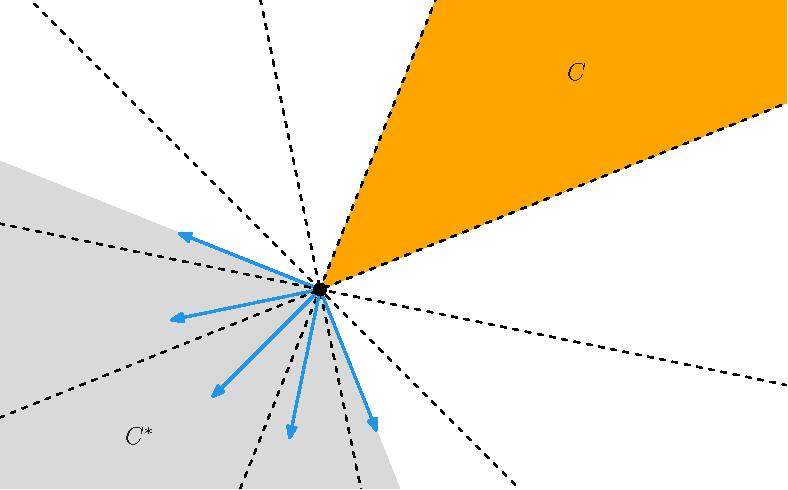
\includegraphics[width=0.7\textwidth]{fig/dual_cone.pdf}
\caption{A cone $K$ and its negative dual cone $-K^*$ (equivalently, its polar
  cone $K^\circ$), which can be easier to visualize. The set $-K^*$ is
  characterized by the normal vectors $y$ to all halfspaces $\{y : y^\T x \leq
  0\}$ containing $K$.}     
\label{fig:dual_cone}
\end{figure}

\section{Dual polyhedra*}
\label{sec:dual_polyhedra}

Recall (as covered in Chapter \ref{sec:polyhedra}), a polyhedron is an
intersection of halfspaces, $P = \{x : Ax \leq b\}$, for a matrix-vector pair 
$A,b$ of compatible dimensions. The \emph{dual polyhedron} to $P$ is defined as    
\index{polyhedron!dual polyhedron}
\index{polytope!dual polytope}
\begin{equation}
\label{eq:dual_polyhedron}
P^* = \{ y : y^\T x \leq 1, \; x \in P \}.
\end{equation}
The set $P^*$ is indeed a polyhedron (an intersection of halfspaces),  
% For example, Corollary 19.2.2 of Rockafellar (1970)
although this may be nonobvious at face value. The developments below will make
it clear that $P^*$ is polyhedral in the case that $P$ is bounded. The unbounded
case is discussed in Exercise \ref{ex:minkowski_weyl}. 
 
Let us assume henceforth that $P$ is bounded polyhedron, which recall we call a
polytope, with $0 \in \interior(P)$. While Theorem \ref{thm:hv_representation},
the main representation theorem for polytopes, can be established directly using 
algebraic arguments, we demonstrate in this section how it can be explained from 
the perspective of polyhedral duality. 

To this end, suppose that we have the H-representation $P = \{ x : Ax \leq
b\}$. Then by definition, 
\begin{align}
\nonumber
P^* &= \{ y : y^\T x \leq 1, \; \text{for all $x$ with $Ax \leq b$} \} \\
\label{eq:v_representation_dual}
&= \bigg\{ \sum_{i=1}^m t_i \frac{a_i}{b_i} : \text{$t_i \geq 0$, for
  $i=1,\dots,m$, and $\sum_{i=1}^m t_i = 1$} \bigg\}.
\end{align}
The second step above can be verified using Farkas' lemma (Exercise
\ref{ex:v_representation_dual}), where $a_1,\dots,a_m \in \R^d$ denote the rows
of $A$, and $b_1,\dots,b_m > 0$ (as $0 \in \interior(P)$). Defining $y_i =
a_i/b_i$, $i = 1,\dots,m$, we have thus produced the dual V-representation $P^*
= \conv\{y_1,\dots,y_m\}$.       

Suppose instead that we have the V-representation $P =
\conv\{x_1,\dots,x_n\}$. Again by definition,  
\begin{align}
\nonumber
P^* &= \big\{ y : y^\T x \leq 1, \; x \in \conv\{x_1,\dots,x_n\} \big\} \\
\label{eq:h_representation_dual}
&= \{ y : y^\T x_i \leq 1, \; i = 1,\dots,n \},
\end{align}
where the second step holds by convexity (Exercise
\ref{ex:h_representation_dual}). In other words, we have produced the dual
H-representation $P^* = \{ y : Xy \leq 1\}$, where $X$ is the matrix with rows
$x_1,\dots,x_n \in \R^d$.    

We have therefore established that the H-representation and V-representation for
polytopes are dual to one another: facets (halfspaces in an H-representation) of
$P$ correspond to vertices (points in a V-representation) of $P^*$, and vice 
versa. This dual relationship can actually be used as a key step in proving
Theorem \ref{thm:hv_representation} in the first place; see Exercise 
\ref{ex:hv_representation_dual}.    

There is in fact even more to be said about the relationship between $P$ and
$P^*$: not only vertices and facets, but all faces of $P$ and $P^*$ obey a
precise one-to-one correspondence. 

\begin{Theorem}
\label{thm:face_duality}
Let $P \subseteq \R^d$ be a polytope with $0 \in \interior(P)$, and let $P^*$ be
its dual polytope in \eqref{eq:dual_polyhedron}. Define a map $\Psi$ from faces
$\cF(P)$ of $P$ to faces $\cF(P^*)$ of $P^*$ by  
\[
\Psi(F) = \{ y \in P^* : y^\T x = 1, \; x \in F \}.
\]
Then $\Psi$ is a bijection. Furthermore, it is inclusion-reversing: $F \subseteq
G \implies \Psi(F) \supseteq \Psi(G)$, and it satisfies $\dim(F) + \dim(\Psi(F))
= d-1$ for all $F \in \cF(P)$. 
\end{Theorem}

This theorem, whose proof is outlined in Exercise \ref{ex:face_duality}, gives
us a rich way of understanding the relation between a polytope $P$ and its dual
$P^*$. Duality provides a representation map $\Psi$, which maps vertices of $P$
to facets of $P^*$, edges (1-faces) of $P$ to ridges ($(d-2)$-faces) of $P^*$,
and so on. In short, the  entire facial structure of $P$ is determined by $P^*$,
and vice versa. A canonical example of a dual polytope pair is given by the
$\ell_1$ and $\ell_\infty$ balls, explored in Exercise
\ref{ex:l1_linf_ball_duality}.    

\section{Polar sets*}
\label{sec:polar_sets}

Given a set $C$, its \emph{polar set} is defined by 
\index{polar set}
\begin{equation}
\label{eq:polar_set}
C^\circ = \{ y : y^\T x \leq 1, \; x \in C \}.
\end{equation}
For a polyhedron $P$, its polar set is simply another name for its dual
polyhedron \eqref{eq:dual_polyhedron}, $P^\circ = P^*$. Moreover, for a cone
$K$, its polar set is in fact the negative dual cone \eqref{eq:dual_cone},
$K^\circ = -K^*$: clearly we have $-K^* \subseteq K^\circ$, and for the opposite
inclusion, take any $y \in K^\circ$, $x \in K$, $t>0$, then observe that $y^\T x  
\leq 1 \implies y^\T (tx) \leq 1 \iff y^\T x \leq 1/t$, thus sending $t \to
\infty$ gives $y^\T x \leq 0$.          

One can check that the polar $C^\circ$ is always a closed convex set. When $C$
itself a closed convex set containing 0, the polar of its polar set is
\begin{equation}
\label{eq:polar_set_polar}
C^{\circ\circ} = C.
\end{equation}
As polarity generalizes duality for both polyhedra and cones, the above fact
implies $P^{**} = P$ for a polyhedron containing the origin, and also $K^{**} =
K$ for a closed convex cone, as claimed earlier in
\eqref{eq:dual_cone_dual}. The fact \eqref{eq:polar_set_polar} can be verified
using the separating hyperplane theorem (Exercise \ref{ex:polar_set_polar}). 

\begin{Example}
The \emph{tangent cone} to a set $C$ at a point $x \in C$ is defined as 
\index{normal cone!dual cone}
\index{tangent cone}
\begin{equation}
\label{eq:tangent_cone}
T_C(x) = \closure \{ y : x + ty \in C, \; \text{for small enough $t>0$} \}. 
\end{equation}
This is a closed cone, but need not be convex in general. However, if $C$ is
convex then $T_C(x)$ is convex too, and in this case it is actually the polar to
the normal cone, $(N_C(x))^\circ = T_C(x)$. Exercise \ref{ex:tangent_cone}
explores these and related details.     
\end{Example}

Polarity and conjugacy share a connection for characteristic functions. By
direct inspection, the conjugate of $I_C$, which recall (Example
\parref{xa:support_function_conjugate}) is the support function $h_C = I^*_C$,
satisfies        
\[
h_C(y) \leq 1 \iff y \in C^\circ.
\]
Moreover, if $C$ is a cone, then we can see from the above that $h_C$ can
only take the values 0 and $\infty$ (since $h_C(y) \leq 1 \implies h_C(ty) = t
h_C(y) \leq 1$ for all $y \in C^\circ$ and $t>0$); more precisely, $h_C$ is 0 
on $C^\circ$ and $\infty$ otherwise, which leads to 
\begin{equation}
\label{eq:support_function_cone}
h_C = I_{C^\circ}.
\end{equation}
That is, the conjugate (support function) of the characteristic function of a
cone is the characteristic function of its polar cone. This fact will be useful
in our discussion of conic duality, next.  
  
% Where do we want to prove conjugate of sum of indicators is conjugate of
% indicator of intersection?  

% Dual in terms of gauge of polar set?

\section{Conic duality*}
\label{sec:conic_duality}

blah blah

% Make sure to mention that conjugate of indicator of convex cone is indicator
% of its polar cone. 

How to write in a unified way?

Write cone program as follows in a way that allows Fenchel duality to be applied
elegantly. For example, min $c^\T x$ subject $Ax + b \in K$

See Theorems 3.2.2 and 3.2.5 in Ben Tal and Nemirovski. This is more general and 
it will be helpful to write this as: min $f(x)$ subject to $h(x) \leq 0$, $Ax =
b$, where $h$ is $K$-convex and $K$ is a regular cone (regular means: closed,
convex, nonempty interior, pointed)

\begin{equation}
\label{eq:primal_conic}
\begin{alignedat}{2}
&\minimize_x \quad && f(x) \\
&\st \quad && h(x) \leq_K 0 \\
& && Ax = b.
\end{alignedat}
\end{equation}

\index{Slater's condition}
\index{strong duality}
\begin{Theorem}
\label{thm:slater_conic}
TODO. MAKE SURE TO GIVE STATEMENTS OF ATTAINMENT SO WE CAN USE THAT IN AN
EARLIER EXERCISE.    

State as in the earlier Slater, that we get strong duality. Then say,
furthermore, when the common optimal value is finite, that this is attained in 
the dual, i.e., dual solution exists. 

% Consider the optimization problem \eqref{eq:primal_problem}, where after 
% relabeling, if needed, we take $h_1, \dots, h_r$ to be inequality constraint
% functions which are affine ($r = 0$ if none are affine). Assume the following.         

% \begin{enumerate}[label=(\roman*)]
% \item The functions $f$ and $h_i$, $i=1,\dots,m$ are convex, and $\ell_j$,
%   $j=1,\dots,k$ are affine; in other words, problem \eqref{eq:primal_problem} is
%   convex, and we can write its equality constraints as $Ax = b$.      

% \item There exists $x \in \relint(D)$, where \smash{$D = \dom(f) \cap
%     \bigcap_{i=r+1}^m \dom(h_i)$} denotes the common effective domain, such that      
%   \begin{equation}
%   \label{eq:slater_condition}
%   h_i(x) \leq 0 \;\, \text{for all $i \leq r$}, \quad
%   h_i(x) < 0 \;\, \text{for all $i \geq r+1$}, \quad 
%   Ax = b.
%   \end{equation}
% \end{enumerate}

% Then strong duality holds: the optimal values $f^\star$ in problem
% \eqref{eq:primal_problem} and $g^\star$ in the corresponding dual problem  
% \eqref{eq:dual_problem} satisfy $f^\star = g^\star$.
\end{Theorem}

\section{Minimax theorems*}
\label{sec:minimax_theorems}

?? consider Bert chap 5.5 or BTN chap 3.4.2 

\section{Existence of minima revisited*}
\label{sec:existence_minima_revisited}

discuss 0 being in int(dom(f)) being equivalent to f* having no directions
of recession.  give nice proposition/theorem about existence of solutions of 
$$
\minimize_\theta \quad g(X \theta) + h_C(x),
$$
where $C$ is a convex set. prove in exercises. specialize to generalized linear
model case, interpret sufficient conditions, and prove theorems in Chapter
\ref{sec:maximum_likelihood} about existence of logistic and Poisson regression
solutions. 

% Lemma 14 here: https://www.stat.berkeley.edu/~ryantibs/papers/genlasuni.pdf 

MAKE Sure to talk about interpretation of logistic interpretation

\SkipTocEntry\section*{Chapter notes}

Polyhedral duality: Chapter 2 of Ziegler, Chapter 3 of Grunbaum.
Polarity: Chapter 14 of Rockafellar, and Chapter 19 for polyhedral theory.

Exercises \ref{ex:dubovitski_milutin_lemma}, \ref{ex:farkas_variations_conic}, 
and \ref{ex:convex_theorem_alternatives_conic} are based on
\cite{bental2023convex} (Chapters 1.2 and 3.2). 
% Exercise \ref{ex:dual_polyhedron} is based on \cite{rockafellar1970convex}
% (Chapter 19).  

\clearpage

\begin{xcb}{Exercises}
\begin{enumerate}[label=\thechapter.\arabic*]
\settowidth{\leftmargini}{00.00.\hskip\labelsep}
\item \label{ex:dual_norm_check}
  Prove that the dual norm \eqref{eq:dual_norm} is indeed a norm on $\R^d$ by
  verifying the following properties:  
  \begin{itemize}
  \item triangle inequality: $\|x+y\|_* \leq \|x\|_* + \|y\|_*$ for all $x,y \in 
  \R^d$;
  \item absolute homogeneity: $\|ax\|_* = |a|\|x\|_*$ for all $a \in \R$ and $x 
  \in \R^d$; and 
\item positive definiteness: $\|x\|_* \geq 0$ for all $x \in \R^d$, with
  equality if and only if $x=0$. 
  \end{itemize}

\item \label{ex:dual_norm_dual1}
  In this exercise, we investigate the dual of the dual of a norm $\|\cdot\|$: 
  \begin{equation}
  \label{eq:dual_norm_dual}
  \|x\|_{**} = \sup_{\|y\|_* \leq 1} \, x^\T y.
  \end{equation}
  Fixing any $x \in \R^d$, we will argue that $\|x\|_{**} = \|x\|$, in two
  steps.  

\begin{enumerate}[label=\alph*.]
\item Prove $\|x\|_{**} \leq \|x\|$ using H{\"o}lder's inequality
  \eqref{eq:holder_inequality}.  

\item Prove $\|x\|_{**} \geq \|x\|$ using the Hahn-Banach theorem. Hint:
  denoting $X = \R^d$, viewed as a vector space equipped with the norm
  $\|\cdot\|$, note that \eqref{eq:dual_norm_dual} can be rewritten as            
  \[
  \|x\|_{**} = \sup \{ F(x) : F \in X^*, \, \|F\|_{\op} \leq 1 \}.
  \]
  Here $X^*$ denotes the dual space of bounded linear functionals (real-valued 
  functions) on $X$, equipped with the norm \smash{$\|F\|_{\op} = \sup_{x \not 
    =  0} \, |F(x)| / \|x\|$.} Now define $L = \{ ax : a \in \R\}$, a
  1-dimensional subspace of $X$, and define $f : L \to \R$ by 
  $f(ax) = a\|x\|$. Show that $f$ is bounded and linear, with unit operator
  norm, hence by the Hahn-Banach theorem there exists a bounded linear
  functional $F$ on $X$ which agrees with $f$ on $L$, and itself has unit
  operator norm. Use this $F$ to show that $\|x\|_{**} \geq \|x\|$.  
\end{enumerate}

\index{norm!subgradients}
\index{dual norm!subgradients}
\item \label{ex:dual_norm_subgradients}
  In this exercise, we will prove Theorem \ref{thm:dual_norm_subgradients}. 

\begin{enumerate}[label=\alph*.] 
\item Prove that $\text{(i)} \iff \text{(iv)}$ using \eqref{eq:dual_norm}.
\item Prove that $\text{(i)} \iff \text{(v)}$ using \eqref{eq:norm_dual2}.
\item Prove that $\text{(ii)} \iff \text{(iv)}$ using
  \eqref{eq:norm_subgradients}, which comes from applying the Danskin-Bertsekas
  theorem \eqref{eq:danskin_bertsekas} to \eqref{eq:dual_norm}.
\item Prove that $\text{(iii)} \iff \text{(v)}$ using
  \begin{equation}
  \label{eq:dual_norm_subgradients}
  \partial \|y\|_* = \{ x : \|x\| \leq 1, \, x^\T y = \|y\|_* \},
  \end{equation}
  which comes from applying the Danskin-Bertsekas theorem
  \eqref{eq:danskin_bertsekas} to \eqref{eq:norm_dual2}. 
\end{enumerate}

\index{lp norm@$\ell_p$ norm!dual norm}
\item \label{ex:lp_norm_dual}
  In this exercise, we prove $(\|\cdot\|_p)_* = \|\cdot\|_q$, as stated in
  Example \parref{xa:lp_norm_dual}, for $p,q \geq 1$ such that $1/p + 1/q = 1$. 
  It suffices to prove $x^\T y \leq \|x\|_p \|y\|_q$ for all $x,y$ (traditional
  H{\"o}lder's inequality, for $\ell_p$ norms), where equality can always be
  obtained for each $x$ (at some $y$). We consider the cases $p = 1$ and $p > 
  1$ separately.            

\begin{enumerate}[label=\alph*.] 
\item Argue directly that $x^\T y \leq \|x\|_1 \|y\|_\infty$, with equality if
  $y_i = \sign(x_i)$, $i = 1,\dots,d$.

\item When $p > 1$, argue first that we can take $\|x\|_p= \|y\|_q = 1$,  
  without any loss of generality. Then argue that $x_i y_i \leq |x_i|^p / p +
  |y_i|^q / q$, using Young's inequality, and sum this up over each $i =
  1,\dots,d$ to arrive at $x^\T y \leq \|x\|_p \|y\|_q$, with equality if
  $|x_i|^p = c |y_i|^q$ for $c > 0$. 
\end{enumerate}

\item \label{ex:scaled_euclidean_norm_dual}
  Consider the optimization problem
  \[
  \maximize \quad y^\T x \quad \st \quad x^\T A x \leq 1. 
  \]
  Prove that the supremum is attained at \smash{$x = A^{-1} y / \sqrt{y^\T
    A^{-1} y}$}, and so \smash{$(\|y\|_A)_* = \sqrt{y^\T A^{-1} y}$}, as stated
  in Exercise \parref{xa:scaled_euclidean_norm_dual}. 

\index{trace norm!dual norm}
\item \label{ex:trace_norm_dual}
  To prove $(\|\cdot\|_{\tr})_* = \|\cdot\|_{\op}$, as stated in Exercise
  \parref{xa:trace_norm_dual}, we will verify that $(\|\cdot\|_{\op})_* = 
  \|\cdot\|_{\tr}$, where to be clear,
  \[
  (\|X\|_{\op})_* = \sup_{\|Z\|_{\tr} \leq 1} \, \langle Z, X \rangle, 
  \]
  and $\langle Z, X \rangle = \tr(Z^\T X)$. We proceed in two steps; in what
  follows, let $X = U \Sigma V^\T$ be the SVD of $X \in \R^{k \times d}$.

\begin{enumerate}[label=\alph*.] 
\item Prove $(\|X\|_{\op})_* \leq \|X\|_{\tr}$ by direct calculation. Hint:
  given any $Z$ such that $\|Z\|_{\op} \leq 1$, argue that 
  \[
  \langle Z, X \rangle = \langle U^\T Z V, \Sigma \rangle = \sum_{i=1}^d u_i^\T
  Z v_i \sigma_{ii}, 
  \]
  where $u_i,v_i$ denote the $i\th$ columns of $U,V$, respectively, for $i =
  1,\dots,d$. Then argue that each $u_i^\T Z v_i \leq 1$, as $u_i,v_i$ have 
  unit $\ell_2$ norm and $\|Z\|_{\op} \leq 1$.

\item Prove $(\|X\|_{\op})_* \geq \|X\|_{\tr}$ by studying $\langle Z, X
  \rangle$ with $Z = U V^\T$. Hint: verify that now  
  \[
  \langle Z, X \rangle = \langle U^\T Z V, \Sigma \rangle = \sum_{i=1}^d
  \sigma_{ii}.
  \]
\end{enumerate}

% Recall that the Schatten $p$-norm on matrices is defined, for $p \geq 1$, by    
% \[
% \|X\|_p =  \|\sigma(X)\|_p,
% \]
% with the right-hand representing the usual $\ell_p$ norm of the vector
% $\sigma(X) = (\sigma_1(X), \dots, \sigma_n(X))$ of singular values of a matrix 
% $X \in \R^{n \times d}$. Consider
% \[
% (\|X\|_p)_* = \sup_{\|Z\|_p \leq 1} \, \langle Z, X \rangle,
% \]
% where $\langle Z, X \rangle = \tr(Z^\T X)$. Prove that $(\|X\|_p)_* =
% \|X\|_q$, where $1/p + 1/q = 1$.   

\item \label{ex:norm_squared_conjugate}
  We will derive some properties associated with the pair of set-valued
  operators   
  \begin{align*}
  d(x) &= \|x\| \cdot \partial \|x\|, \\
  d^*(y) &= \|y\|_* \cdot \partial \|y\|_*.
  \end{align*}

\begin{enumerate}[label=\alph*.] 
\item Prove that $\|x\| = \|y\|_*$, for $y \in d(x)$.
\item Prove that $x^\T y = \|x\|^2$, for $y \in d(x)$. 
\item For $f(x) = \frac{1}{2} \|x\|^2$, prove that $\partial f(x) = d(x)$. 
\item For $f^*(y) = \sup_x \, \{ y^\T x - f(x) \}$, prove that the supremum
  defining $f^*(y)$ is achieved for $y \in d(x)$. Plug this in, and use parts a
  and b, to verify \eqref{eq:norm_squared_conjugate}. 
\item Prove that $d(x) = \argmax_y \, \{ x^\T y - \frac{1}{2} \|y\|_*^2 \}$, and 
  $d^*(y) = \argmax_x \, \{ y^\T x - \frac{1}{2} \|x\|^2 \}$. 
\item Prove that $y \in d(x) \iff x \in d^*(y)$.
\end{enumerate}

\item \label{ex:dual_norm_dual2}
  Consider the optimization problem 
  \[
  \minimize_z \quad \|z\| \quad \st \quad z = x,
  \]
  whose optimal criterion value is $f^\star = \|x\|$. Show that its Lagrange 
  dual problem is 
  \[
  \maximize_u \quad u^\T x \quad \st \quad \|u\|_* \leq 1,
  \]
  whose optimal criterion value is $g^\star = \|x\|_{**}$. Argue that strong 
  duality holds, $f^\star = g^\star$, which translates to $\|x\|_{**} = \|x\|$. 

\item \label{ex:dual_norm_dual3}
  Use \eqref{eq:norm_squared_conjugate}, and the fact that $f^{**} = f$ for
  closed convex $f$, as in \eqref{eq:double_conjugate_reduction}, to verify
  $\|x\|_{**} = \|x\|$.  

\index{lasso!dual problem}
\item \label{ex:lasso_fenchel_dual}
  For \smash{$f(z) = \frac{1}{2} \|y-z\|_2^2$}, prove either by direct
  calculation or calculus rules for conjugacy that \smash{$f^*(u) = \frac{1}{2}
    \|y+u\|_2^2 - \frac{1}{2} \|y\|_2^2$}. Use this to show that Fenchel
  duality, as given in Example \parref{xa:fenchel_norm}, reproduces the lasso 
  dual in \eqref{eq:lasso_dual}.

\index{support vector machine!hinge form}
\index{support vector machine!dual problem}
\item \label{ex:svm_fenchel_dual}
  Consider the SVM in hinge form, for labels $y_i \in \{ -1, 1\}$ and features
  $x_i \in \R^d$, $i=1,\dots,n$,     
  \begin{equation}
  \label{eq:svm_hinge2}
  \minimize_{\beta_0,\beta} \quad C \sum_{i=1}^n \big[1 - y_i(\beta_0 + x_i^\T 
  \beta)\big]_+ + \frac{1}{2} \|\beta\|_2^2.
  \end{equation}
  We simplify our study, in preparation for examining Fenchel duality, by
  omitting the intercept term $\beta_0$. Denote by $y \in \R^n$ the label
  vector, $X \in \R^{n \times d}$ the feature matrix (with $i\th$ row $x_i^\T$),
  and \smash{$\tilde{X} = \diag(y) X$}. Then the above problem (without
  intercept) can be recast as      
  \begin{equation}
  \label{eq:svm_hinge3}
  \minimize_\beta \quad f(\tilde{X} \beta) + \frac{1}{2} \|\beta\|_2^2, 
  \end{equation}
  where $f(z) = C \sum_{i=1}^n (1-z_i)_+$. To reproduce the dual
  \eqref{eq:svm_dual}, we proceed in steps. 

\begin{enumerate}[label=\alph*.] 
\item Prove by direct calculation that $f^*(u) = 1^\T u \cdot I_{[-C,0]^n}(u)$. 

\item Use Fenchel duality, as given in Example \parref{xa:fenchel_norm_squared}, 
  to prove that the dual of \eqref{eq:svm_hinge3} is
  \begin{alignat*}{2}
  &\maximize_u \quad && 1^\T u - \frac{1}{2} \|\tilde{X}^\T u\|_2^2 \\
  &\st && u \in [0,C]^n.
  \end{alignat*}

\item Adapt the arguments in the previous parts to accommodate the intercept in
  the original problem \eqref{eq:svm_hinge2}, and show that the resulting
  Frenchel dual reproduces \eqref{eq:svm_dual}. Hint: the presence of intercept
  will require you to compute the conjugate of \smash{$(\beta_0, \beta) \mapsto 
    \frac{1}{2} \|\beta\|_2^2$}.    
\end{enumerate}

\item When is dual of dual problem the primal problem? Describe a class of
  problems for which this holds, using Fenchel duality.  

% \item \label{ex:dual_cone_dual}
%   Given an arbitrary cone $K$, consider the dual of its dual cone:  
%   \[
%   K^{**} = \{x : x^\T y \geq 0, \; y \in K^*\}.
%   \]
%   Prove that $K^{**}$ is the intersection of all closed halfspaces containing
%   $K$, and therefore, if $K$ is closed and convex, then $K^{**} = K$,   
%   verifying \eqref{eq:dual_cone_dual}. Hint: recall
%   \eqref{eq:halfspace_intersection} from Exercise
%   \ref{ex:affine_minorant_revisited}.   

\item Let $K_1,\dots,K_m$ be cones, and $K = K_1 \cap \dots \cap K_m$. Prove
  that 
  \[
  K^* \supseteq \closure(K_1^* + \cdots + K_m^*).
  \]
  Prove additionally that if each of the cones $K_1,\dots,K_m$ are closed, then
  equality holds above. Hint: use the strict separating hyperplane theorem, from
  Exercise \ref{ex:farkas_lemma}.

\item \label{ex:dubovitski_milutin_lemma}
  Let $K_1,\dots,K_m$ be closed convex cones, where $K_1 \cap \interior(K_2) 
  \cap \cdots \cap \interior(K_m) \not= \emptyset$. Prove that $K_1 ^* + \cdots
  + K_m^*$ is closed, and hence by the last exercise, $K^* = K_1^* + \cdots
  + K_m^*$. This is known as the \emph{Dubovitski-Milutin lemma}. Hint: consider
  a sequence $y_j = \sum_{i=1}^k y_{ij}$, with $y_{ij} \in K_i^*$ for $j =
  1,2,3,\dots$ and each $i$, with $y_j \to y$ as $j \to \infty$. It remains to
  show that $y \in K_1^* + \cdots + K_m^*$. For this, use the existence of $x
  \in K_1 \cap \interior(K_2) \cap \cdots \cap \interior(K_m)$ to show that
  $y_{ij}$, $j = 1,2,3,\dots$ is a bounded sequence for each $i$, and therefore, 
  passing to a subsequence if needed, it has a subsequence converging to a point
  in $K_i^*$. 
  % Proposition 1.2.7 in Ben-Tal and Nemirovski (2023) 

\item \label{ex:farkas_variations_conic} 
  In this exercise, we will show that the Dubovitski-Milutin lemma, studied in
  the last exercise, leads to an important variation on Farkas' lemma. This will 
  slightly generalize the result from Exercise \ref{ex:farkas_variations} part
  b, which was a key tool used in proving the convex theorem of alternatives
  from Exercise \ref{ex:convex_theorem_alternatives}. Given $A \in \R^{k \times
    d}$, $b \in \R^k$, $g \in \R^d$, $h \in \R$, and a convex set $D \subseteq
  \R^d$, with $b \geq 0$ and $0 \in \interior(D)$, consider two statements:       
  \begin{itemize}
  \item for all $x \in D$, it holds that $Ax \leq b \implies g^\T x \leq h$;  
  \item there exists $\mu \in \R^k$ such that $\mu \geq 0$ and $\mu^\T (Ax - b) 
    \geq g^\T x - h$ for all $x \in D$.
  \end{itemize}
  We will prove that these two statements are equivalent in what follows.
  % Lemma 3.2.1 in Ben-Tal and Nemirovski (2023)
  
\begin{enumerate}[label=\alph*.]
\item Prove that the second statement implies the first.

\item To prove that the first statement implies the second, start by defining 
  \[
  K_1 = \closure \Big\{ (x,t) \in \R^d \times \R: t > 0, \, x/t \in D \Big\}
  \quad \text{and} \quad K_2 = \Big\{ (x,t) \in \R^d \times \R: Ax \leq tb
  \Big\}.  
  \]
  Show that these are closed convex cones, with $\interior(K_1) \cap K_2 \not= 
  \emptyset$. 

\item Define $f = (g,-h) \in \R^{d+1}$, and show that $f^\T (x,t) \leq 0$ for
  all $(x,t) \in K_1 \cap K_2$.  

\item Use Exercise \ref{ex:dubovitski_milutin_lemma} to argue that we can
  decompose $f = \psi + \phi$, where $\psi^\T(x,t) \leq 0$ for all $x \in K_1$,
  and $\phi^\T (x,t) \leq 0$ for all $x \in K_2$.

\item Use Exercise \ref{ex:farkas_variations} part a to show that there exists
  $\mu \geq 0$ such that $[A \, -b]^\T \mu = \phi$, in other words, $\phi^\T
  (x,t) = \mu^\T (Ax - tb)$ for all $x,t$. Use this to prove the desired result.       
\end{enumerate}
  
\item \label{ex:v_representation_dual}
  To verify \eqref{eq:v_representation_dual}, argue that the inclusion
  $\supseteq$ follows directly, whereas the inclusion $\subseteq$ follows using
  the Farkas' lemma variation from Exercise \ref{ex:farkas_variations} part b
  (or Exercise \ref{ex:farkas_variations_conic} with $D = \R^d$). Hint: fixing
  $y$ such that $Ax \leq b$ implies $y^\T x \leq 1$; we know that there exists  
  $\mu \geq 0$ such that $\mu^\T (Ax - b) \geq y^\T x - 1$ for all $x \in 
  \R^d$. Show that this implies $y = A^\T \mu$, and $\mu^\T b \leq 1$.
  We can then reparametrize, using $b_1,\dots,b_m > 0$, since $0 \in
  \interior(P)$, to obtain the desired statement. 

\item \label{ex:h_representation_dual}
  To verify \eqref{eq:h_representation_dual}, argue that the inclusion
  $\subseteq$ follows directly, whereas the inclusion $\supseteq$ follows
  by convexity of the set $\{x : y^\T x \leq 1\}$ for a given $y$.

\item \label{ex:hv_representation_dual}
  In this exercise, we step through a proof of the main representation theorem,
  Theorem \ref{thm:hv_representation}, for polytopes. We treat each direction 
  separately. 

\begin{enumerate}[label=\alph*.]
\item Suppose $P = \{x : Ax \leq b\}$ is an H-representation and $P$ is
  bounded. Use the fact that $P$ has a finite number of faces (Exercise
  \ref{ex:face_structure} part f), along with the Krein-Milman theorem
  (Exercise \ref{ex:extreme_points} part b), to show that $P =
  \conv\{x_1,\dots,x_n\}$ for vertices $x_1,\dots,x_n$.

\item Suppose $P = \conv\{x_1,\dots,x_n\}$ is a V-representation. Show that the
  dual polytope $P^*$ has an H-representation, then use the argument from part a
  applied to $P^*$, and duality once again along with $P^{**} = P$ by
  \eqref{eq:polar_set_polar}, to form an H-representation for $P$.    
\end{enumerate}

\item \label{ex:face_duality}
  This exercise outlines the proof of Theorem \ref{thm:face_duality}. It is
  trivial to check that $\Psi(\emptyset) = P^*$ and $\Psi(P) = \emptyset$, and
  we restrict our attention to a proper face $F \in \cF(P)$.  

% Following Theorem 4 in Chapter 3.4 of Grunbaum (2003)

\begin{enumerate}[label=\alph*.]
\item Let $x_0 \in \relint(F)$, and $F^* = \{ y \in P^* : y^\T x_0 = 1 \}$.
  Prove that $\Psi(F) = F^*$, and so $\Psi(F)$ is indeed a face of
  $P^*$. Hint: suppose that $\Psi(F) \not= F^*$, and take $y_0 \in F^* \setminus
  \Psi(F)$. Argue there exists $x_1 \in F$ such that $y_0^\T x_1 < 1$. Use $x_0
  \in \relint(F)$ to argue that $y_0^\T x_0 < 1$. 

\item Prove the inclusion-reversing property: given $G \supseteq F$, we have
  $\Psi(G) \subseteq \Psi(G)$.  

\item Prove the dimensionality property: $\dim(F) + \dim(\Psi(F)) = d-1$.  
\end{enumerate}

\item \label{ex:l1_linf_ball_duality}
  Consider the $\ell_1$ and $\ell_\infty$ balls in $\R^d$,
  \[
  P = \bigg\{ x : \sum_{i=1}^d |x_i| \leq 1 \bigg\} \quad \text{and} \quad 
  Q = \bigg\{ x : \max_{i=1,\dots,d} \, |x_i| \leq 1 \bigg\}. 
  \]
  In geometry these are often referred to as the \emph{cross-polytope} and
  \emph{hypercube}, respectively.  

\begin{enumerate}[label=\alph*.]
\item Prove directly with a counting argument that the number of $k$-faces of
  $P$ is $2^{k+1} {d \choose k+1}$.  

\item Prove directly with a counting argument that the number of $k$-faces of
  $Q$ is $2^{d-k} {d \choose d-k}$. 

\item Prove that $P^* = Q$, and check that the relationship between the faces of
  $P$ and $Q$ from Theorem \ref{thm:face_duality} is consistent with parts a and
  b above. 
\end{enumerate}

\item \label{ex:minkowski_weyl}
  We say that a set $C \subseteq \R^d$ is \emph{finitely generated} provided
  there exists $x_1,\dots,x_n \in \R^d$ and $k \leq n$ such that $C = 
  \conv\{x_1,\dots,x_k\} + \cone\{x_{k+1},\dots,x_n\}$, or in other words  
  \[
  C = \bigg\{
  \sum_{i=1}^n t_i x_i : \text{$t_i \geq 0$, for $i=1,\dots,n$, and
    $\sum_{i=1}^k t_i = 1$} \bigg\}.  
  \]
  When $k = n$, note that $C$ reduces to the convex hull of $x_1,\dots,x_n$,
  which is bounded, but when $k < n$, the set $C$ will be unbounded. A 
  generalization of Theorem \ref{thm:hv_representation}, sometimes referred to
  as the \emph{Minkowski-Weyl theorem}, is as follows: 
  \index{Minkowski-Weyl theorem}
  \index{polyhedron!dual polyhedron}
  \begin{equation}
  \label{eq:hv_representation_generalized}
  \text{a set $P$ is a polyhedron if and only if it is finitely generated.}
  \end{equation}
  % For example, Theorem 19.1 in Rockafellar (1970)
  In what follows, we will use this generalization to prove certain facts about
  polyhedra. Denote by $P = \{x : Ax \leq b\} \subseteq \R^d$ a polyhedron, and
  $f : \R^d \to \R^m$ a linear transformation.     

\begin{enumerate}[label=\alph*.]
\item Show that the preimage $f^{-1}(P)$ of $P$ under $F$ is a polyhedron. 

\item Show that the image $f(P)$ of $P$ under $F$ is a polyhedron. Hint: use
  \eqref{eq:hv_representation_generalized}. 

\item Show that the dual $P^*$ defined in \eqref{eq:dual_polyhedron} is a 
  polyhedron. Hint: use \eqref{eq:hv_representation_generalized}.
\end{enumerate}

\item \label{ex:polar_set_polar}
  Given an arbitrary set $C$, consider the polar of its polar set:
  \[
  C^{\circ\circ} = \{ x : x^\T y \leq 1, \; y \in C^\circ \}.
  \]
  In this exercise, we verify \eqref{eq:polar_set_polar}, assuming $C$ is closed
  and convex with $0 \in C$.
  
\begin{enumerate}[label=\alph*.] 
\item Prove that $C \subseteq C^{\circ\circ}$.
\item Prove that $C \supseteq C^{\circ\circ}$. Hint: fix $x_0 \notin C$, and
  argue that $x_0 \notin C^{\circ\circ}$ using the strict version of the
  separating hyperplane theorem given in Exercise \ref{ex:farkas_lemma}. Use $0
  \in C$ to show that the separating hyperplane can be expressed as $y^\T x_0 >
  1$ and $y^\T x < 1$ for all $x \in C$.
\end{enumerate}

\item \label{ex:tangent_cone}
  This exercise studies the tangent cone \eqref{eq:tangent_cone} to a set $C$ at
  a point $x \in C$. 

\begin{enumerate}[label=\alph*.] 
\item Give an example to show that $T_C(x)$ can be nonconvex.
\item For convex $C$, prove that $T_C(x)$ is convex. 
\item For convex $C$, prove that $N_C(x) = (T_C(x))^\circ$. Hint: prove the two 
  directions of inclusion ($\subseteq$ and $\supseteq$) separately. Only one 
  will require convexity.     
\item For convex $C$, use part c, the fact that $N_C(x)$ is always closed,
  convex, and contains 0, and \eqref{eq:polar_set_polar} to establish that
  $(N_C(x))^\circ = T_C(x)$.     
\end{enumerate}

\item \label{ex:convex_theorem_alternatives_conic}
  just guide them through the conic theorem of alternatives from 3.2.2 in BTN
  and the conic slater condition in the main text, by generalizing earlier
  proofs, and using the above Farkas lemma variation

\item \label{ex:trace_norm_semidefinite} 
  



% \begin{enumerate}
% \item[(a, 5pts)]
% Show that computing the trace norm of a matrix, i.e., computing $\| X \|_{\tr}$, can be expressed as the following (convex) optimization problem:
% \begin{equation}
% \begin{array}{ll}
% \maximizewrt{Y \in \mathbb{R}^{m \times n}} & \tr(X^T Y) \\
% \subjectto & 
% \left[
% \begin{array}{cc}
% I_m & Y \\
% Y^T & I_n
% \end{array}
% \right]
% \succeq 0,
% \end{array}
% \label{eq:aa:primal}
% \end{equation}
% where $I_p$ is the $p \times p$ identity matrix.  (By the way, problem \eqref{eq:aa:primal} is a semidefinite program; more on this in part (d) below.)

% Hint: think about using the ``Schur complement'' somewhere here.  A good reference for this might be Section A.5.5 in the ``Convex Optimization'' book, by Stephen Boyd and Lieven Vandenberghe.

% \item[(b, 5pts)]
% Show that the dual problem associated with \eqref{eq:aa:primal} can be expressed as
% %\begin{equation}
% %\begin{array}{ll}
% %\minimizewrt{\substack{W_{1} \in \symm^{m}, \\ W_{2} \in \symm^{n}}} & (1/2) ( \tr(I_m W_1) + \tr(I_n W_2) ) \\
% %\subjectto &
% %\left[
% %\begin{array}{cc}
% %W_1 & X \\
% %X^T & W_2
% %\end{array}
% %\right]
% %\succeq 0,
% %\end{array}
% %\label{eq:aa:dual}
% %\end{equation}
% \begin{equation}
% \begin{array}{ll}
% \minimizewrt{\substack{W_{1} \in \symm^{m}, \\ W_{2} \in \symm^{n}}} & \tr(W_{1}) + \tr(W_{2}) \\
% \subjectto & 
% \left[
% \begin{array}{cc}
% W_{1} & (1/2) X \\
% (1/2) X^T & W_{2}
% \end{array}
% \right]
% \succeq 0,
% \end{array}
% \label{eq:aa:dual}
% \end{equation}
% where, just to remind you, $\symm^p$ is the space of $p \times p$ real, symmetric matrices.

% \item[(c, 2pts)]
% Show that the optimal values for problems \eqref{eq:aa:primal} and \eqref{eq:aa:dual} are equal to each other, and that both optimal values are attained.

% \item[(d, 5pts)]
% In the \textit{matrix completion problem}, we want to find a matrix $X \in \reals^{m \times n}$ of low rank that is close, in a squared error sense, to some observed matrix $Z \in \reals^{m \times n}$.  We do not assume that all of the entries of $Z$ are observed, so we will look at the squared error over $Z$'s observed entries only, which we store in a set $\Omega$ of (observed) row and column indices.  Putting all this together leads us to the following (convex) optimization problem:
% \begin{equation}
% \begin{array}{ll}
% \minimizewrt{X \in \mathbb{R}^{m \times n}} & \sum_{(i,j) \in \Omega} ( X_{ij} - Z_{ij} )^2 + \lambda \| X \|_{\tr},
% \end{array}
% \label{eq:aa:mtxcomp}
% \end{equation}
% with tuning parameter $\lambda > 0$.

% Show that problem \eqref{eq:aa:mtxcomp} can be expressed as a semidefinite program of the form
% \begin{equation*}
% \begin{array}{ll}
% \minimizewrt{x \in \mathbb{R}^p} & c^T x \\
% \subjectto & x_1 A_1 + \cdots + x_p A_p \preceq B,
% \end{array}
% \end{equation*}
% for some fixed $c, B, A_i, \; i=1,\ldots,p$.

% Hint: you will probably need to ruse each of the above parts (in different ways) here.

\item Exercise on plurality of dual problems?

\end{enumerate}
\end{xcb}